%%%%%%%%%%%%%%%%%%%%%%%%%%%%%%%%%%%%%%%%%%%%%%%%%%%%%%%%%%%
% --------------------------------------------------------
% Tau
% LaTeX Template
% Version 2.4.1 (22/05/2024)
%
% Author: 
% Guillermo Jimenez (memo.notess1@gmail.com)
% 
% License:
% Creative Commons CC BY 4.0
% --------------------------------------------------------
%%%%%%%%%%%%%%%%%%%%%%%%%%%%%%%%%%%%%%%%%%%%%%%%%%%%%%%%%%%
\documentclass[9pt,a4paper,twoside]{tau-class/tau}
%----------------------------------------------------------
% TITLE
%----------------------------------------------------------
\journalname{计算物理\uppercase\expandafter{\romannumeral3}}
\title{含时薛定谔方程的数值解法}
%\CJKfamily{SimSun}
%----------------------------------------------------------
% AUTHORS, AFFILIATIONS AND PROFESSOR
%----------------------------------------------------------

\author[a,1]{Author}
%\author[b,2]{Author Two}
%\author[b,c,3]{Author Three}

%----------------------------------------------------------

\affil[a]{武汉大学,物理科学与技术学院}
%\affil[b]{Affiliation of author two}
%\affil[c]{Affiliation of author three}

%\professor{Professor/Authority or other information}

%----------------------------------------------------------
% FOOTER INFORMATION
%----------------------------------------------------------

\institution{Wuhan University}
\footinfo{Homework\uppercase\expandafter{\romannumeral4}}
\theday{December, 2024}
\leadauthor{Author}
\course{计算物理\uppercase\expandafter{\romannumeral3}}

%----------------------------------------------------------
% ABSTRACT AND KEYWORDS
%----------------------------------------------------------

\begin{abstract}    

\end{abstract}

%----------------------------------------------------------

\keywords{薛定谔方程,切比雪夫多项式,紧束缚模型}

%----------------------------------------------------------
\begin{document}
\onecolumn
\nolinenumbers
    \maketitle 
    \thispagestyle{firststyle}
	%\tauabstract 
    \taukeywords
    \tableofcontents
    \linenumbers 
    
%----------------------------------------------------------
\begin{multicols}{2}
\nolinenumbers
\section{薛定谔方程}
\paragraph{}薛定谔方程在量子力学中占有十分重要的位置,根据量子力学的六个假定,正是薛定谔方程决定了物理体系随时间演变的规律\cite{QUANTUM}。
\begin{tauenv}[frametitle=薛定谔方程]
    \begin{align}
        i\hbar\dv{ }{t}|\varphi(t)\rangle=\hat{H}|\varphi(t)\rangle
    \end{align}
\end{tauenv}
由此可知,只要给出了初态$|\varphi(0)\rangle$就足以决定此后任意时刻的态$|\varphi(t)\rangle$。因此在物理体系演变过程中发没有任何不确定性。
\subsection{原子单位制}
\paragraph{}在数值计算中,一些常数,比如$\hbar,m_e,\varepsilon$等,不仅使得公式非常繁琐,并且在实际的计算当中增加了复杂度,同时由于这些常数往往很大或者很小,大大降低了计算精度,容易出现数值溢出。为此,人们往往使用原子单位制重写方程:\cite{sb}
\begin{tabular}{c|c}
    \toprule
    \multicolumn{2}{c}{原子单位制} \\[2pt]
    \hline
    质量&$m_e=9.1094\times 10^{-31}kg$\\
    电荷&$e=1.6022\times 10^{-19}C$\\
    角动量&$\hbar=1.0546\times 10^{-43}J\cdot s$\\
    介电常数&$4\pi\varepsilon_0=1.1127\times 10^{-10}F\cdot m^{-1}$\\
    长度&$a_0=\frac{4\pi\varepsilon_0\hbar^2}{m_ee^2}=5.2918\times 10^{-11}m$\\
    能量&$Hartree=\frac{m_ee^2}{(4\pi\varepsilon_0)^2\hbar}=4.3597\times 10^{-18}J$\\
    \bottomrule
\end{tabular}
\\
在合适的单位制下(事实上此处也并非原子单位制,而是令$\frac{\hbar^2}{2m}=0$),二维的薛定谔方程改写为:
\begin{equation}
    \begin{gathered}
        i\dv{}{t}|\varphi(t)\rangle=\hat{H}|\varphi(t)\rangle\\
        \hat{H}=-\pdv[2]{}{x}-\pdv[2]{}{y}+V(\mathbf{r})\label{se}
    \end{gathered}
\end{equation}
\section{数值解法}
\subsection{离散化}
显然,数值求解薛定谔方程之前需要对方程\ref{se}进行离散化,设$\delta$为网格的间距,用$\psi_{l,k}(t)$近似地表示$\varphi(l\delta,k\delta,t)$。用最简单的差分近似替代关于x,y的导数:
\begin{align}
    \frac{\partial^2\psi(x,y,t)}{\partial x^2}&\approx \frac{\psi(x+\delta,y,t)-2\psi(x,y,t)+\psi(x-\delta,y,t)}{\delta^2}\\
    &=\delta^{-2}[\psi_{l+1,k}-2\psi_{l,k}+\psi_{l+1,k}]
\end{align}
一维的离散薛定谔方程可以写成
\begin{align*}
    \pdv{\psi(t)}{t}=-i\{-\delta^{-2}[\psi_{l+1}+\psi_{l-1}]+v_{l}\}
\end{align*}
哈密顿量可以写为矩阵的形式
\[ \hat{H} = \left[
\begin{array}{cccc}
v_1 & -\delta^2 & \ldots & 0\\
-\delta^2  & v_1 & \ldots & 0\\
\vdots & \vdots & \ddots & \vdots\\
0 & 0 & \ldots & v_l\\
\end{array} \right] \]
同理,二维的薛定谔方程可以写为\\
\begin{align}
    \pdv{\psi(t)}{t}=-i\{-\delta^{-2}[\psi_{l+1,k}+\psi_{l-1,k}+\psi_{l,k+1}+\psi_{l,k-1}]+v_{l,k}\}
    \label{2d}
\end{align}
其中$v_{l,k}=V(x,y)-4$。如果我们将$\psi_{lk}$按照先排列x方向后y方向的方式堆积成一个列向量,即:
\begin{equation}
    \psi_{lk}=\psi_{n},n=(k-1)L+l
\end{equation},
那么$\hat{H}$仍然可以写成一个矩阵:
\[ \hat{H} = \left[
\begin{array}{cccccc}
v_{11} & -\delta^2  & \cdots &-\delta^2  &\cdots & 0\\
-\delta^2  & v_{12} & \cdots& \cdots & \cdots & 0\\
\vdots & \vdots & \vdots & \vdots& \vdots& \vdots \\
-\delta^2 &0& \cdots &\cdots & \cdots& 0\\
\vdots &\vdots &\vdots & \vdots &  \vdots & \vdots \\
0 & 0 & \cdots & \cdots & -\delta^2  &v_{LK}\\
\end{array} \right] \]
方程\ref{2d}也可以理解为一个粒子在$N=L\times K$的二维网格中传播,这种理解对于处理更加复杂的哈密顿量是十分重要的。
\begin{equation}
    \begin{gathered}
        \hat{H}=-t\sum_{n}^{N}(c^{\dag}_{n+1}c_{n}+c^{\dag}_{n}c_{n+1}+c^{\dag}_{n+L}c_{n}+c^{\dag}_{n}c_{n+L}-W\sum_{n}^{N}\epsilon_nc^{\dag}_nc_n)\\
        |\varphi(t)\rangle=\sum_{n=1}^{N+1}\psi_n(t)c^{\dag}_n|0\rangle
    \end{gathered}
    \label{cc}
\end{equation}
$c^{\dag},c$是产生湮灭算符。对比方程\ref{2d}和\ref{cc},不难发现$t=\delta^{-2},W\epsilon_n=v_n$。
\subsection{矩阵指数}
与普通的微分方程类似,矩阵微分方程有解析解\cite{De1996}:
\begin{equation}
    \begin{aligned}
        i\dv{\hat{U}(t)}{t}=\hat{H}(t)\hat{U}\\
        \hat{U}(t)=e^{-i\hat{H}t}\hat{U}(0)
    \end{aligned}
\end{equation}
问题的关键在于求出$e^{-i\hat{H}t}$。矩阵指数由Taylor级数定义:
\begin{align}
    e^{xH}=\sum_{n=0}^{\infty}\frac{x^n}{n!}H^n
\end{align}
尽管这样的展开在数学上是非常重要的,但是在实际计算中没有意义,一方面存储矩阵需要占用大量的内存,对计算资源造成巨大的浪费;另一方面,Taylor展开无法满足波函数模方守恒的要求:
\begin{equation}
    \begin{aligned}
        &\langle \varphi(0)|\varphi(0)\rangle=\langle \varphi(t)|\varphi(t)\rangle\\
        &\neq\langle\varphi(0)|(I+itH-\frac{t^2}{2}H+\cdots)(I-itH-\frac{t^2}{2}H+\cdots)|\varphi(0)\rangle
    \end{aligned}
\end{equation}
为此我们引入切比雪夫多项式方法计算$e^{-i\hat{H}t}$
\subsection{切比雪夫多项式}
为了演化波函数,需要对时间演化算子进行数值展开,由于哈密顿量是稀疏的,所以可以方便地使用Chebyshev多项式进行展开,这种方法对求解含时薛定谔方程是无条件稳定的。假设$x\in[-1,1]$,
\begin{equation}
    e^{-izx}=J_0(z)+2\sum_{m=1}^{\infty}(-i)^mJ_m(z)T_m(x)
\end{equation}
其中$J_m$是m阶贝塞尔函数,$T_m$是第一类切比雪夫多项式。$T_m(x)$可以由递归关系求解:
\begin{equation}
    T_{m+1}(x)=2xT_{m}-T_{m-1}
\end{equation}
为了利用切比雪夫多项式方法,我们需要将$\hat{H}$缩放为$\tilde{H}=\hat{H}\Vert H\Vert$,使$\tilde{H}$的特征值分布在$[-1,1]$。
\begin{equation}
    |\varphi(t)\rangle=\{J_0(\tau)+2\sum_{m=1}^{\infty}(-i)^mJ_m(\tau)\hat{T}_m(\tilde{H})\}|\varphi(0)\rangle
\end{equation}
$\tau=t\cdot\Vert H\Vert$。在实际计算中不需要存储$\hat{T}_m$,而是由递归关系直接计算波函数:
\begin{equation}
    \hat{T}_{m+1}(\tilde{H})\varphi(0)=2\tilde{H}\hat{T}_{m}(\tilde{H})\varphi(0)-\hat{T}_{m-1}(\tilde{H})\varphi(0)
\end{equation}
除了时间演化算子$e^{-it\hat{H}}$外,其他算子也可以使用类似方法,展开为切比雪夫多项式的级数。
\begin{equation}
    f(x)=\frac{1}{2}c_0T_0(x)+\sum_{m}c_mT_m(x)
\end{equation}
系数定义为
\begin{equation}
    c_m=\frac{2}{\pi}\int_{-1}^{1}\frac{\dd{x}}{\sqrt{1-x^2}}f(x)T_m(x)
\end{equation}
令$x=\cos{\theta}$,并带入上式,可以得到:
\begin{equation}
    \begin{aligned}
        c_m=\frac{2}{\pi}\int_{0}^{\pi}f(\cos{\theta})\cos(m\theta)\dd{\theta}\\
        =Re[\frac{2}{\pi}\sum_{n=0}^{N-1}f(\cos\frac{2\pi n}{N})e^{i\frac{2\pi n}{N}m}]
    \end{aligned}
\end{equation}
因此可以使用快速傅里叶变换计算出$c_k$。以Fermi-Dirac算符为例:
\begin{equation}
    \begin{aligned}
        f(\hat{H})&=\frac{ze^{-\beta\hat{H}}}{1+ze^{-\beta\hat{H}}},\\
        \text{where}\quad\beta&=\frac{1}{k_BT},z=e^{\beta\mu}
    \end{aligned}
\end{equation}
我们定义$\tilde{\beta}=\beta\cdot\Vert\hat{H}\Vert$。根据前面的讨论:
\begin{equation}
    f(\tilde{H})=\sum_{m=0}^{\infty}c_mT_m(\tilde{H})
\end{equation}
\section{高斯波包}
\subsection{Theory}
本节我们将用上面提到的方法计算一个高斯波包通过波导时波函数随时间的演化。初始的波函数设置为:
\begin{align}
    \Psi(x,y,t_0)=Ae^{-\frac{x^2}{4\sigma _x^2}-\frac{y^2}{4\sigma _y^2}+ik_0x}
\end{align}
为了合理地设置网格数量和演化时间等参数,我们有必要讨论一个波包自由传播时的解析理论。为简单起见,我们首先考虑一维的情形:
\begin{equation}
    \Psi(x,0)=Ae^{-\frac{x^2}{4\sigma^2}+ik_0x}
\end{equation}
由归一化求得$A=(\frac{1}{2\pi\sigma^2})^\frac{1}{4}$叠加原理告诉我们,自由粒子的波函数时各种波矢的平面波的叠加:
\begin{equation}
    \Psi(x,t)=\frac{1}{\sqrt{2\pi}}\int_{-\infty}^{\infty}g(k)e^{i(kx-\omega t)}dk
\end{equation}
我们已知t=0时刻的波函数,于是可以由傅里叶变换求出$g(k)$:
\begin{equation}
    \begin{aligned}
        g(k)&=\frac{1}{\sqrt{2\pi}}\int \Psi(x,0)e^{-ikx}\dd{dx}\\
        &\frac{A}{\sqrt{2\pi}}\int e^{-\frac{x^2}{4\sigma^2}e^{-i(k-k_0)x}\dd{x}}\\
        &\frac{A}{\sqrt{2\pi}}\int e^{-\frac{1}{(2\sigma)^2}(x+2i(k-k_0)\sigma^2)^2-(k-k_0)^2\sigma^2}\dd{x}
    \end{aligned}
\end{equation}
利用留数的性质可以证明,若满足$-\frac{\pi}{4}<Arg(\alpha)<\frac{\pi}{4}$:
\begin{equation}
    \begin{aligned}
        I(\alpha,\beta)&=\int_{-\infty}^{\infty}e^{-\alpha^2(\xi+\beta)^2}\dd{\xi}\\
        &=I(\alpha,0)=\frac{\sqrt{\pi}}{\alpha}
    \end{aligned}
\end{equation}
于是:
\begin{equation}
    \Psi(x,t)=\frac{\sqrt{2\sigma}}{(2\pi)^{3/4}}\int_{-\infty}^{\infty}e^{-(k-k_0)^2\sigma^2}e^{ikx}\dd{k}
\end{equation}
不难证明t时刻波包的形状仍然为高斯波包。再来计算t时刻波函数的模方:
\begin{equation}
    |\Psi(x,t)|^2=\sqrt{\frac{2}{\pi a^2}}\frac{1}{\sqrt{1+\frac{4\hbar^2t^2}{m^2a^4}}}\exp\{-\frac{2a^2(x-\frac{\hbar k_0t}{m})^2}{a^4+\frac{4\hbar^2t^2}{m^2}}\}
\end{equation}
$a=2\sigma$。此时波包的最大值位于$x_M$:
\begin{equation}
    x_M=\frac{\hbar k_0}{m}t
\end{equation}
求出波包的群速度:
\begin{equation}
    V_G=\dv{x_M}{t}=\frac{\hbar k_0}{m}
\end{equation}
二维波包穿过狭缝时衍射波的角宽度近似满足:
\begin{equation}
    2\theta\approx\frac{2\lambda}{\Delta y}
\end{equation}
\end{multicols}
\subsection{Result}
\begin{figure*}[h!]
    \centering
    \begin{subfigure}{0.3\linewidth}
        \includegraphics[width=\linewidth]{10/0}
    \end{subfigure}
    \begin{subfigure}{0.3\linewidth}
        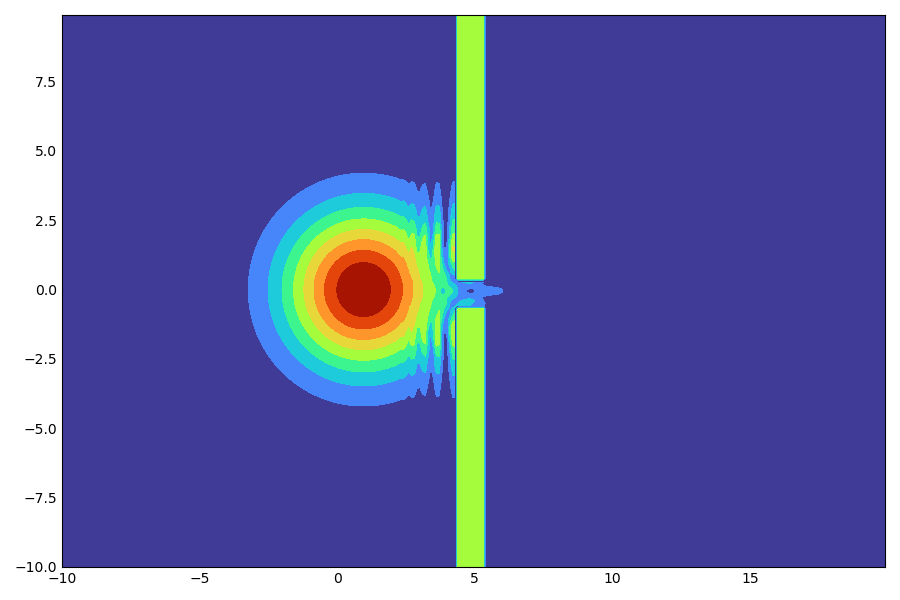
\includegraphics[width=\linewidth]{10/100}
    \end{subfigure}
    \begin{subfigure}{0.3\linewidth}
        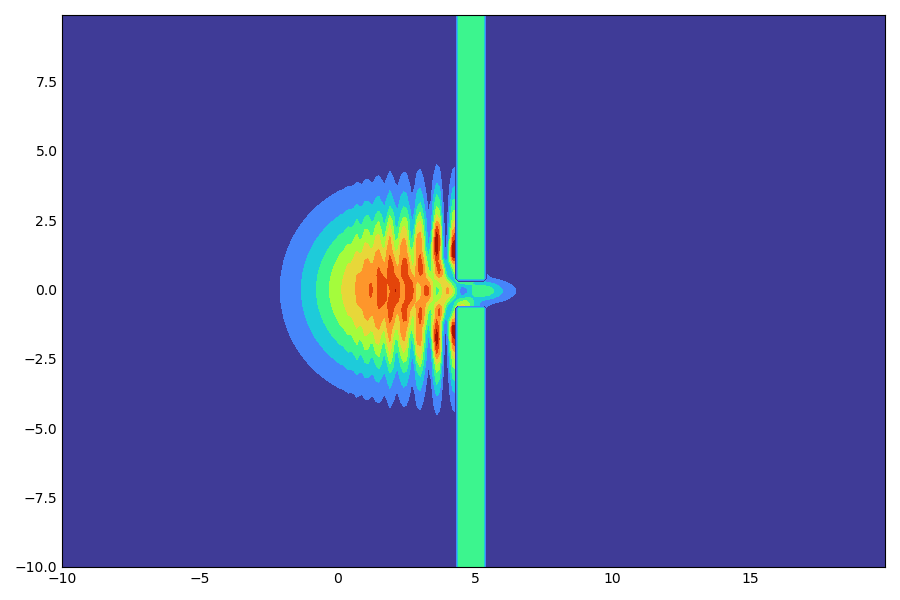
\includegraphics[width=\linewidth]{10/200}
    \end{subfigure}
    \begin{subfigure}{0.3\linewidth}
        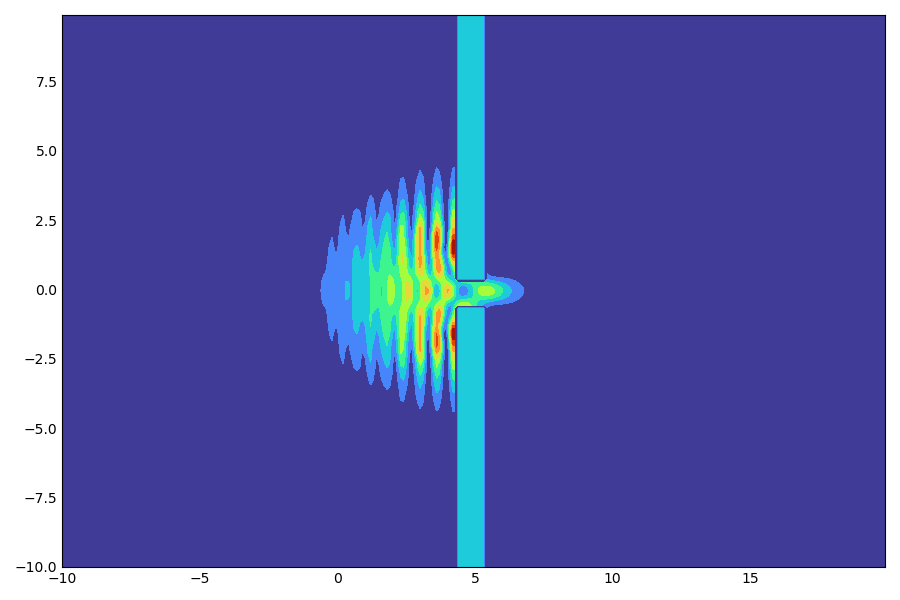
\includegraphics[width=\linewidth]{10/300}
    \end{subfigure}
    \begin{subfigure}{0.3\linewidth}
        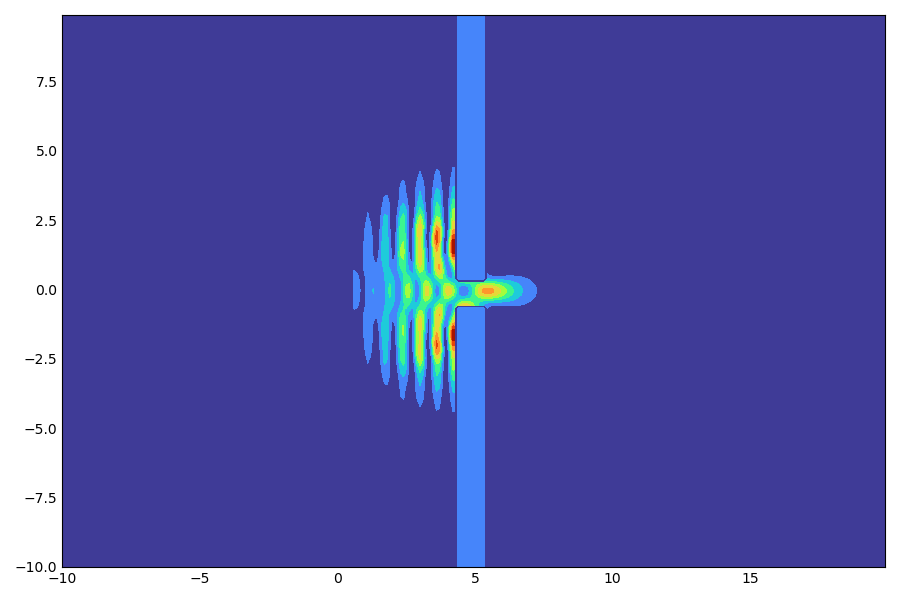
\includegraphics[width=\linewidth]{10/400}
    \end{subfigure}
    \begin{subfigure}{0.3\linewidth}
        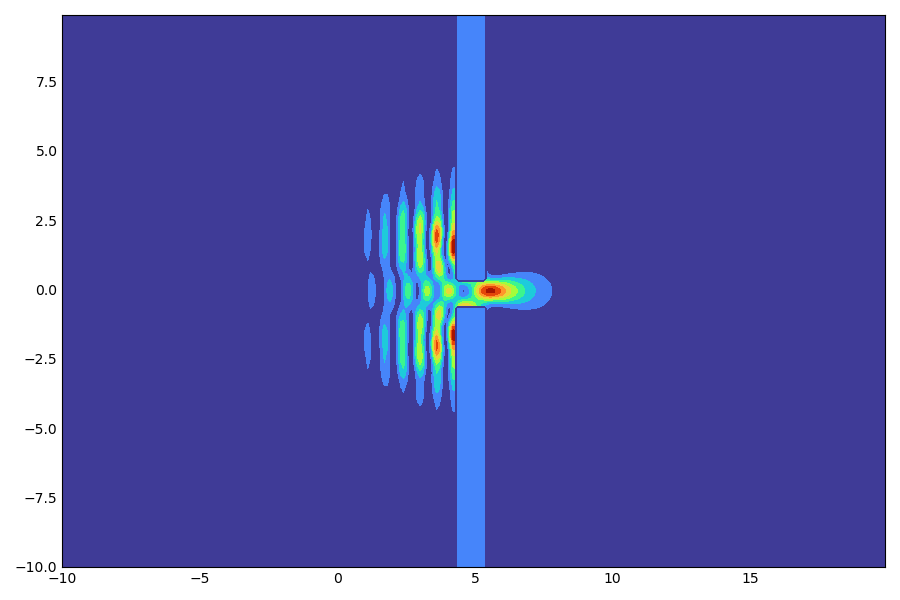
\includegraphics[width=\linewidth]{10/500}
    \end{subfigure}
    \begin{subfigure}{0.3\linewidth}
        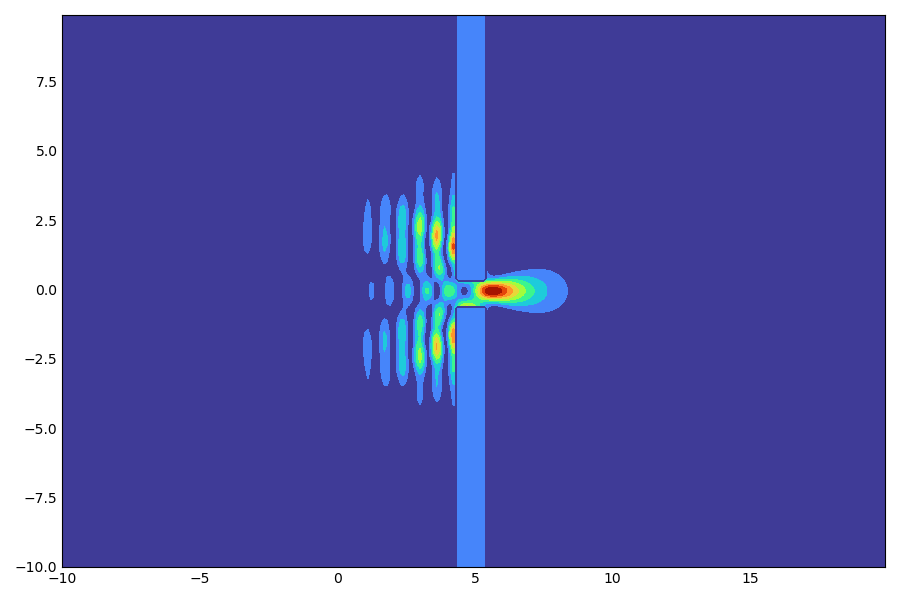
\includegraphics[width=\linewidth]{10/600}
    \end{subfigure}
    \begin{subfigure}{0.3\linewidth}
        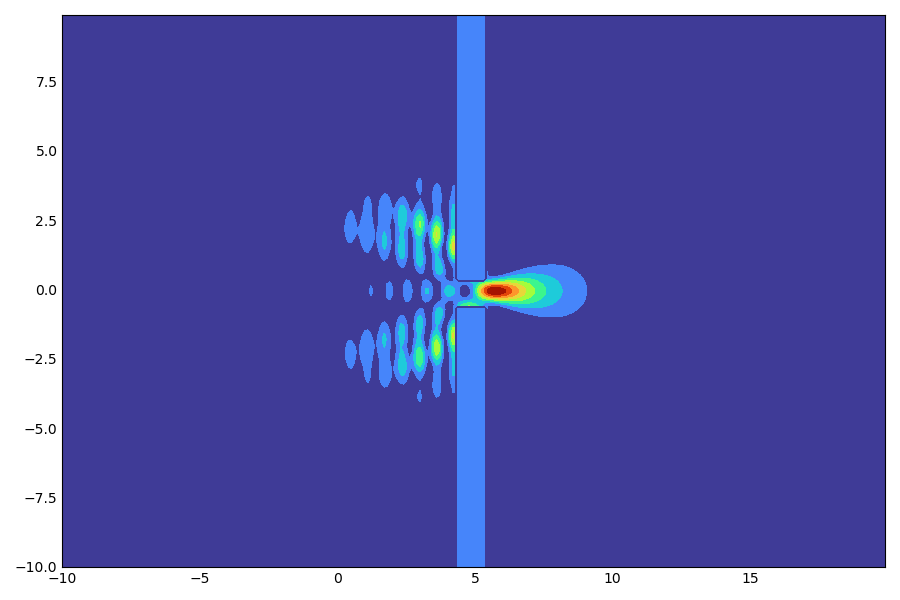
\includegraphics[width=\linewidth]{10/700}
    \end{subfigure}
    \begin{subfigure}{0.3\linewidth}
        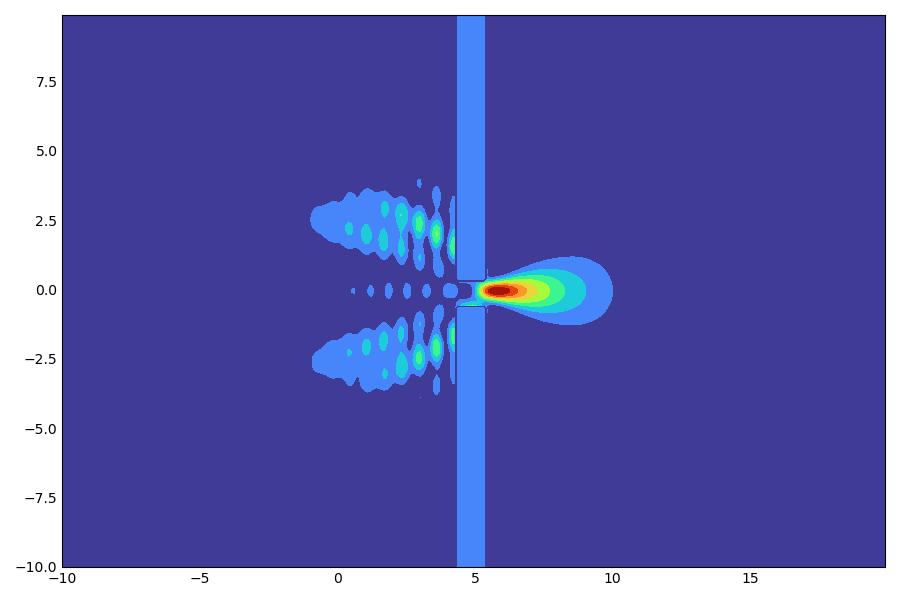
\includegraphics[width=\linewidth]{10/800}
    \end{subfigure}
    \begin{subfigure}{0.3\linewidth}
        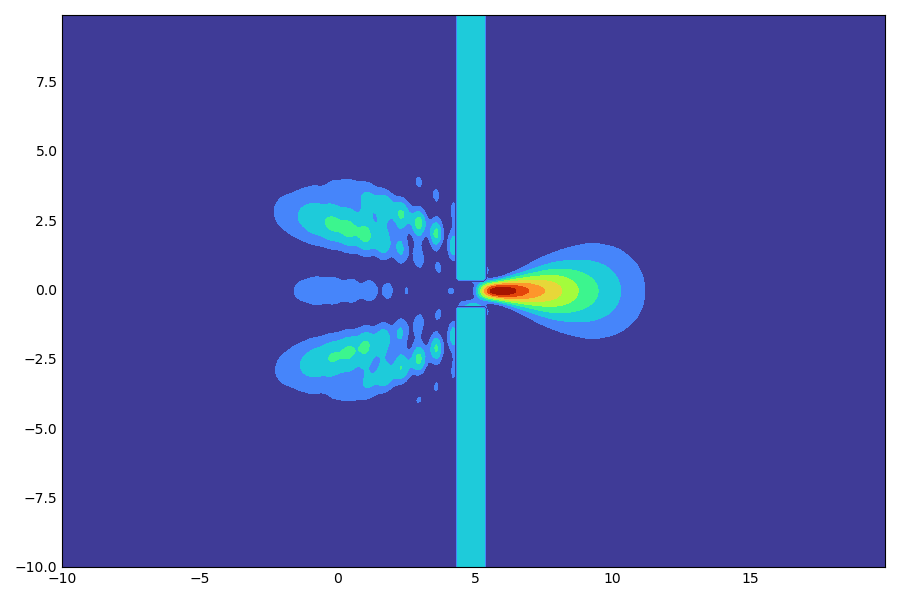
\includegraphics[width=\linewidth]{10/900}
    \end{subfigure}
    \begin{subfigure}{0.3\linewidth}
        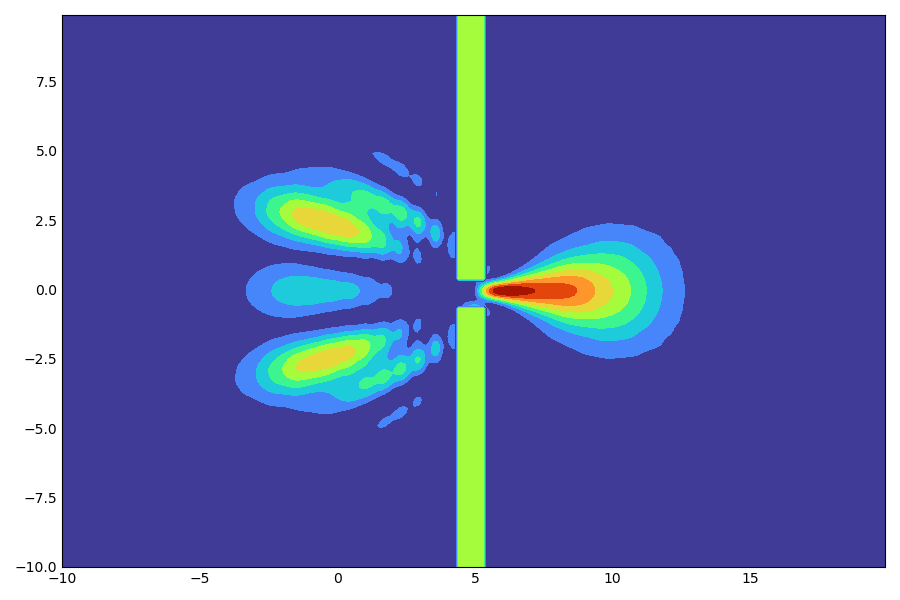
\includegraphics[width=\linewidth]{10/1000}
    \end{subfigure}
    \begin{subfigure}{0.3\linewidth}
        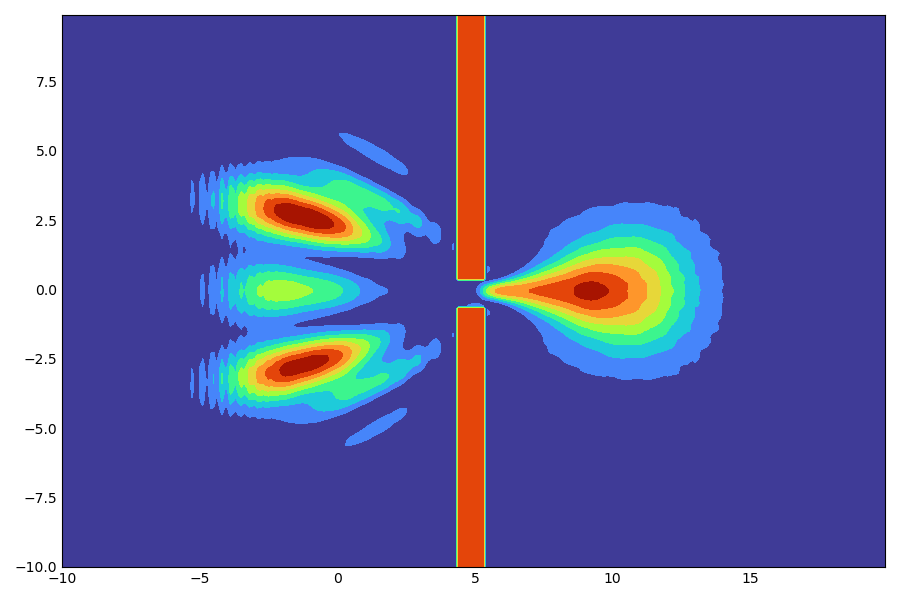
\includegraphics[width=\linewidth]{10/1100}
    \end{subfigure}
    \caption{$\Delta y=20\delta,t\in[0,1100]$}
\end{figure*}
\begin{figure*}[h]
    \centering
    \begin{subfigure}{0.3\linewidth}
        \includegraphics[width=\linewidth]{5/0}
    \end{subfigure}
    \begin{subfigure}{0.3\linewidth}
        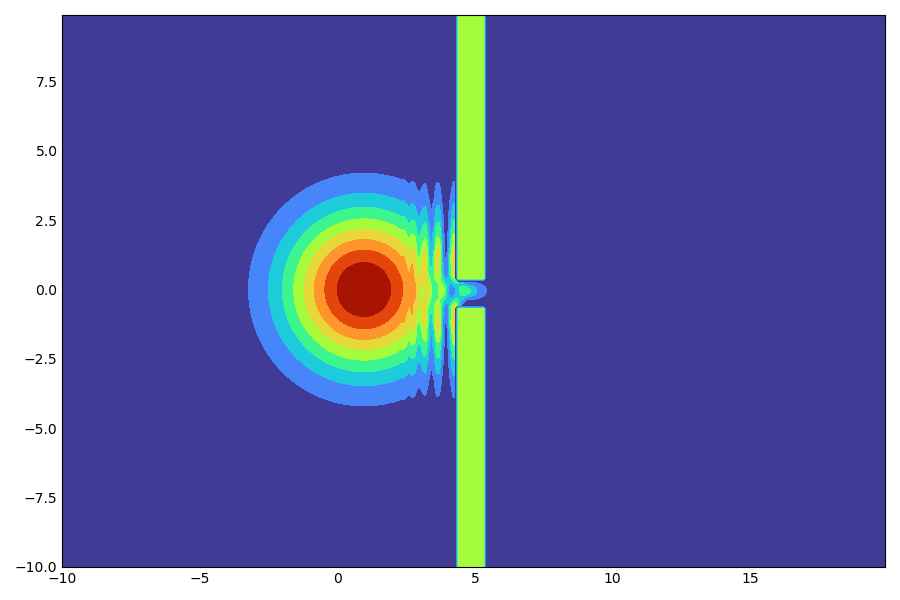
\includegraphics[width=\linewidth]{5/100}
    \end{subfigure}
    \begin{subfigure}{0.3\linewidth}
        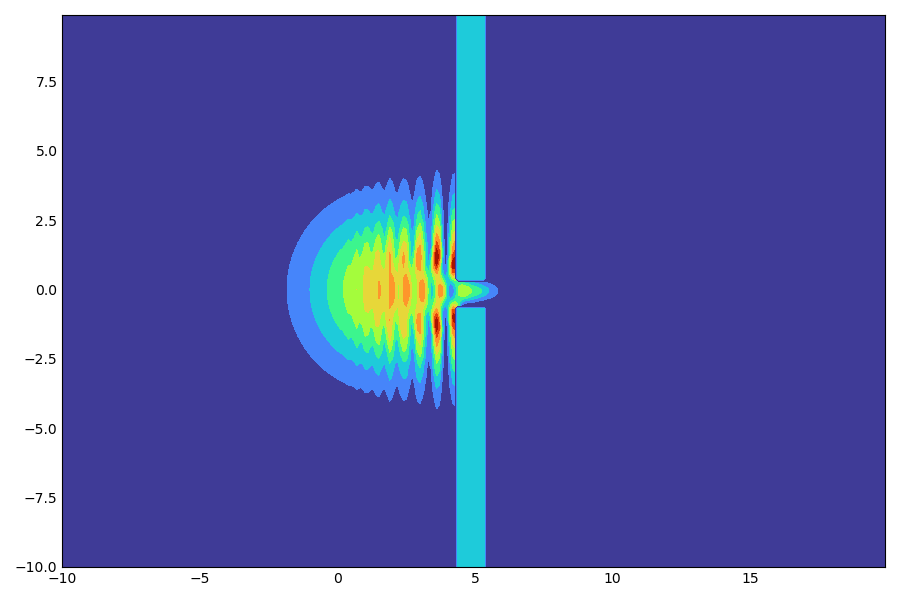
\includegraphics[width=\linewidth]{5/200}
    \end{subfigure}
    \begin{subfigure}{0.3\linewidth}
        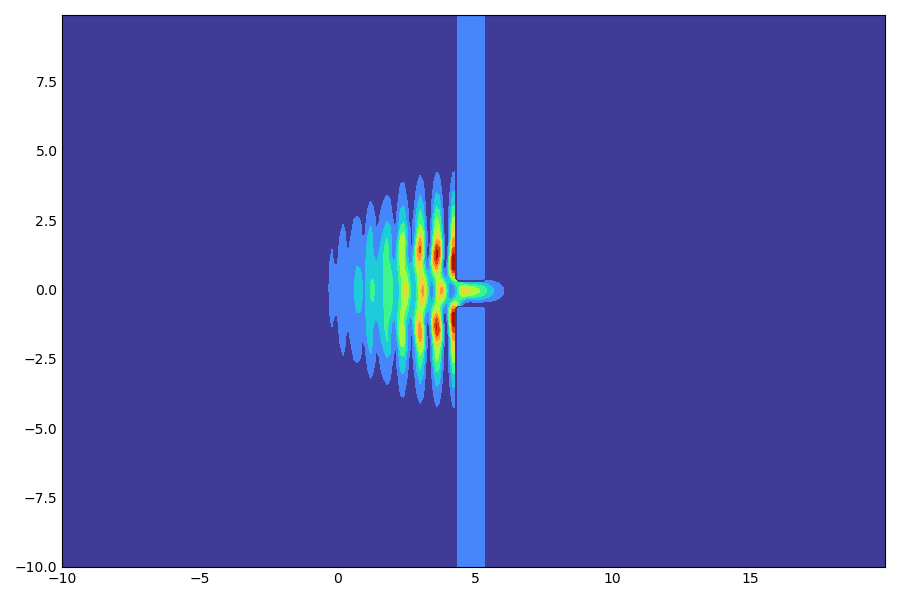
\includegraphics[width=\linewidth]{5/300}
    \end{subfigure}
    \begin{subfigure}{0.3\linewidth}
        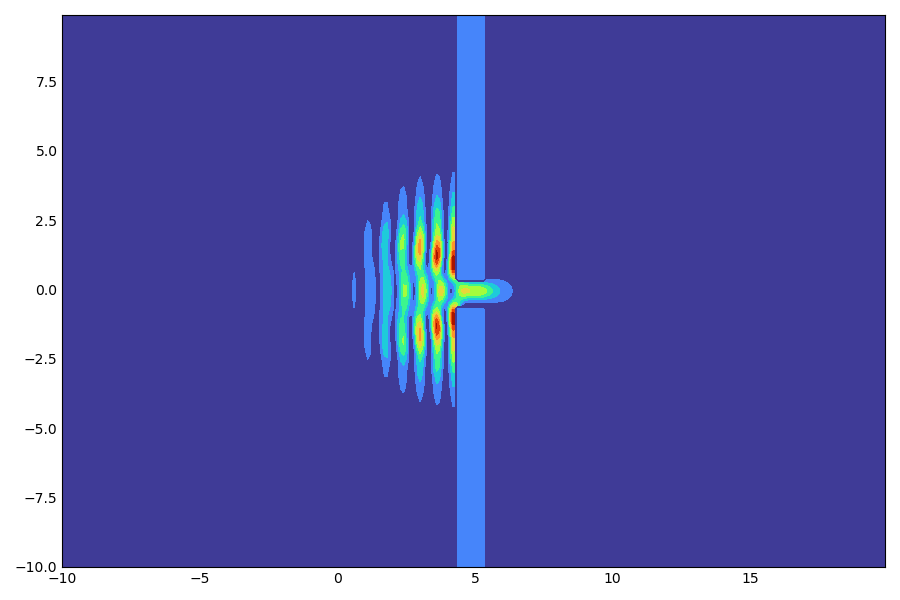
\includegraphics[width=\linewidth]{5/400}
    \end{subfigure}
    \begin{subfigure}{0.3\linewidth}
        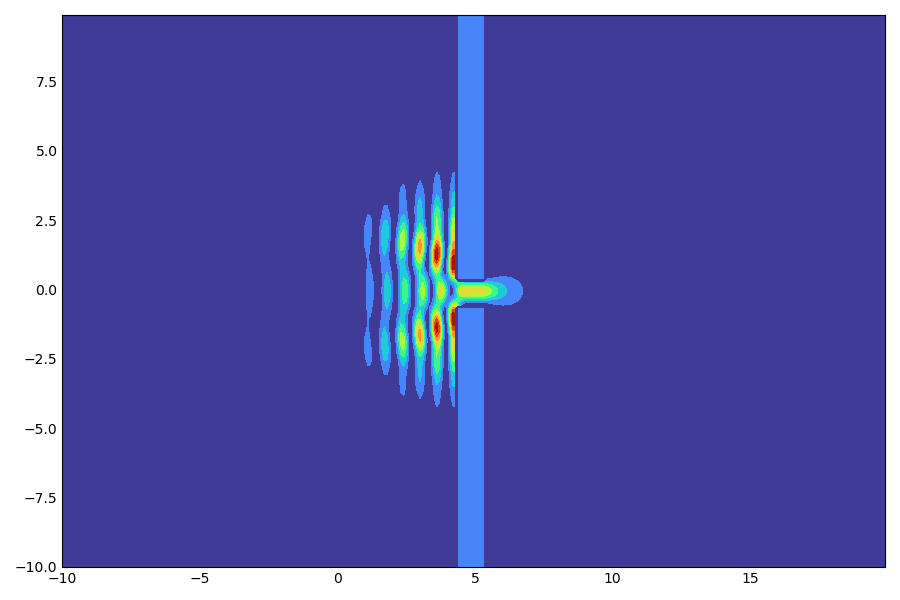
\includegraphics[width=\linewidth]{5/500}
    \end{subfigure}
    \begin{subfigure}{0.3\linewidth}
        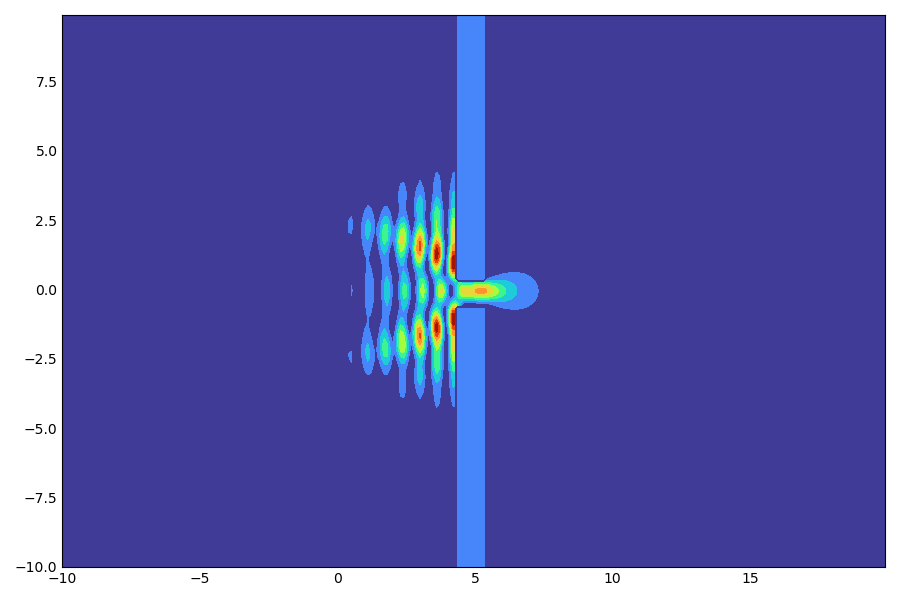
\includegraphics[width=\linewidth]{5/600}
    \end{subfigure}
    \begin{subfigure}{0.3\linewidth}
        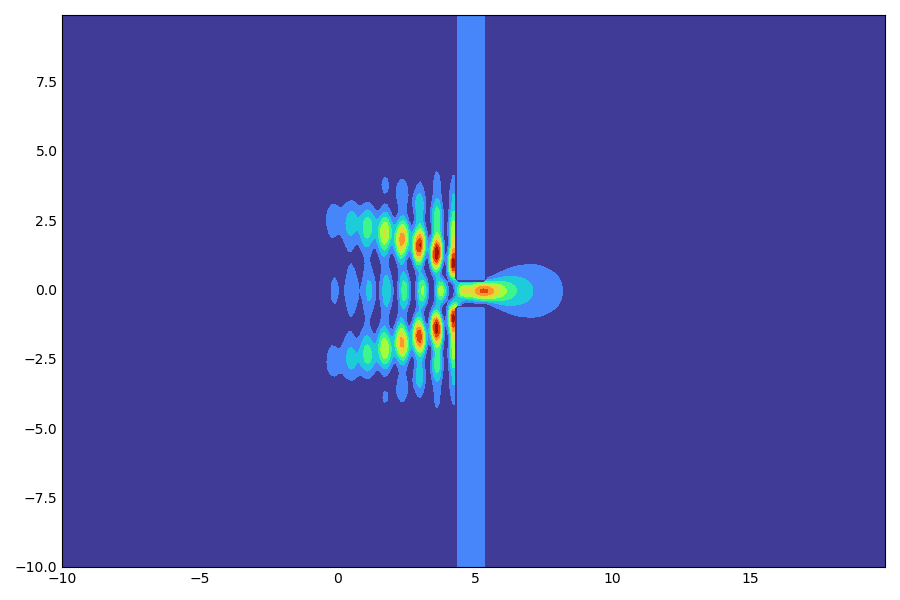
\includegraphics[width=\linewidth]{5/700}
    \end{subfigure}
    \begin{subfigure}{0.3\linewidth}
        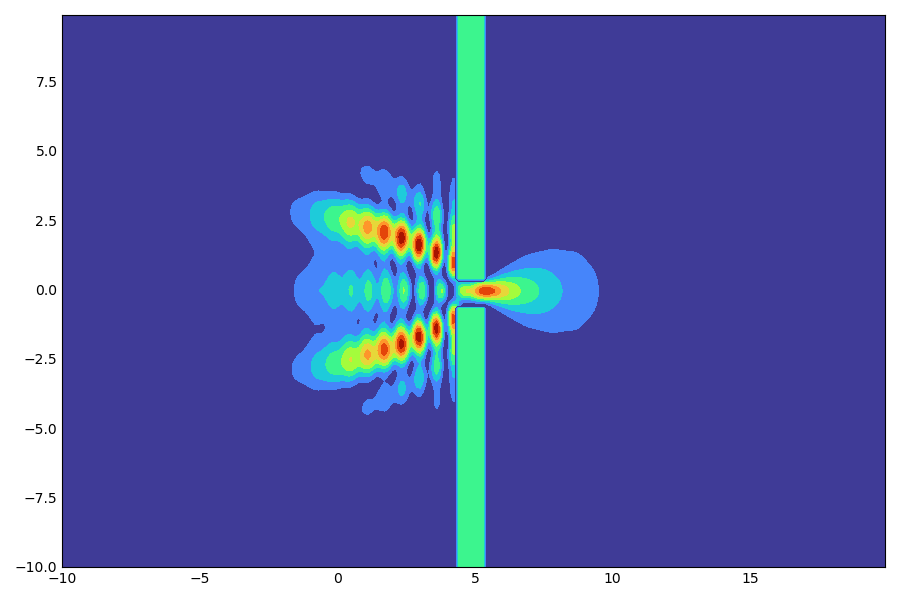
\includegraphics[width=\linewidth]{5/800}
    \end{subfigure}
    \begin{subfigure}{0.3\linewidth}
        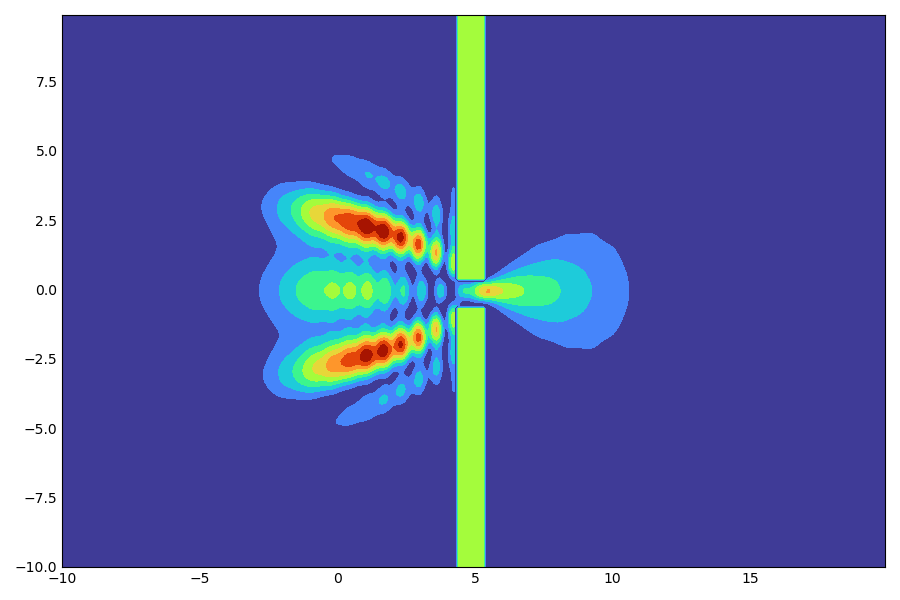
\includegraphics[width=\linewidth]{5/900}
    \end{subfigure}
    \begin{subfigure}{0.3\linewidth}
        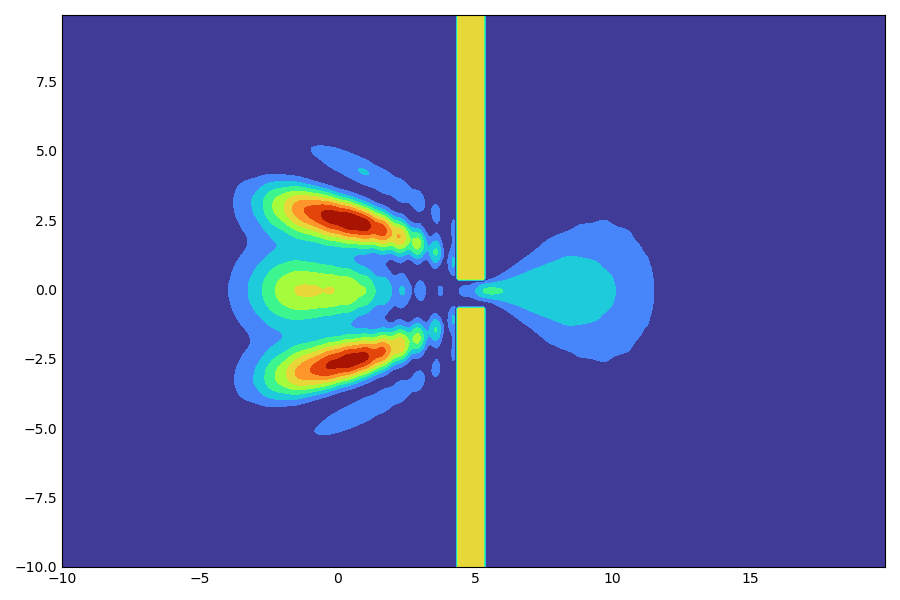
\includegraphics[width=\linewidth]{5/1000}
    \end{subfigure}
    \begin{subfigure}{0.3\linewidth}
        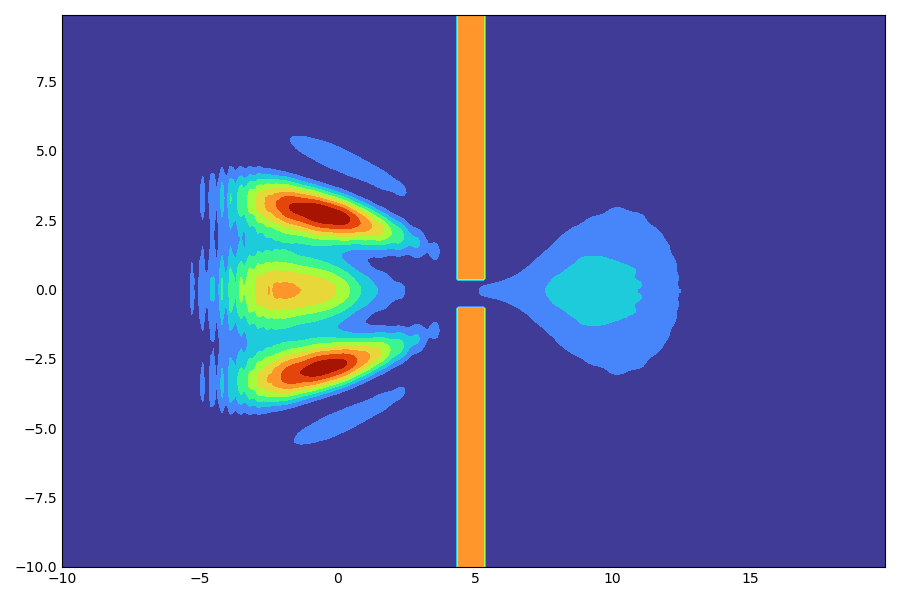
\includegraphics[width=\linewidth]{5/1100}
    \end{subfigure}
    \caption{$\Delta y=10\delta,t\in[0,1100]$}
\end{figure*}
\begin{figure*}[h]
    \centering
    \begin{subfigure}{0.3\linewidth}
        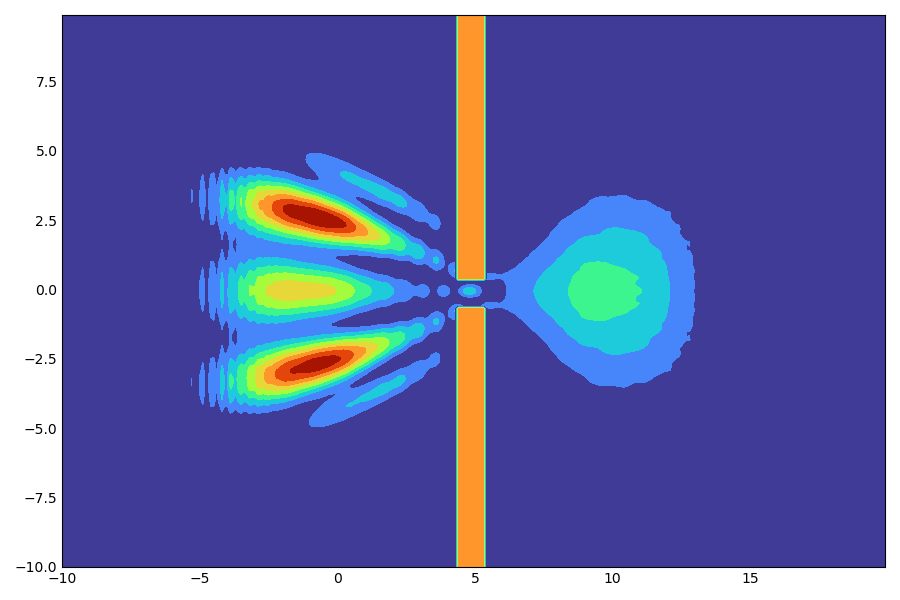
\includegraphics[width=\linewidth]{5/8}
    \end{subfigure}
    \begin{subfigure}{0.3\linewidth}
        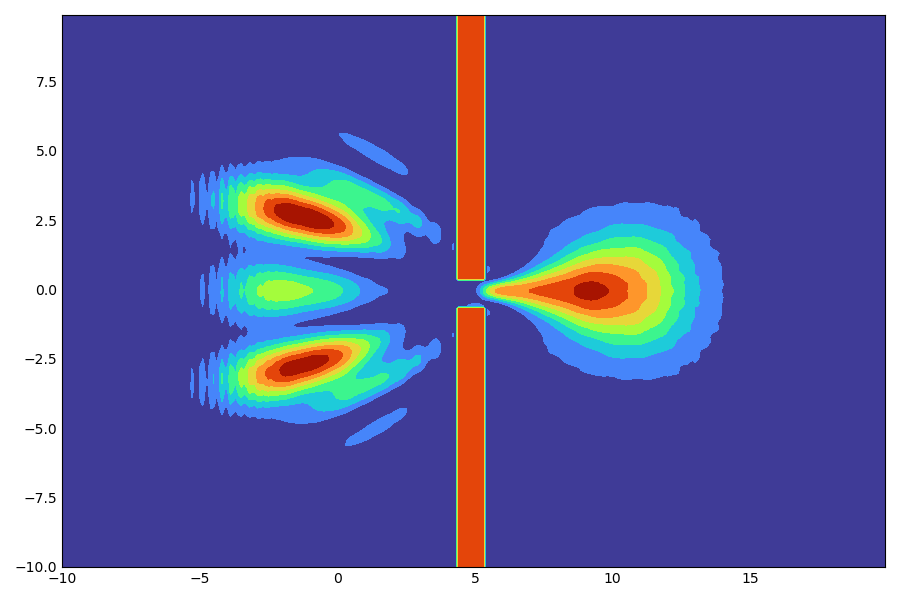
\includegraphics[width=\linewidth]{5/10}
    \end{subfigure}
    \begin{subfigure}{0.3\linewidth}
        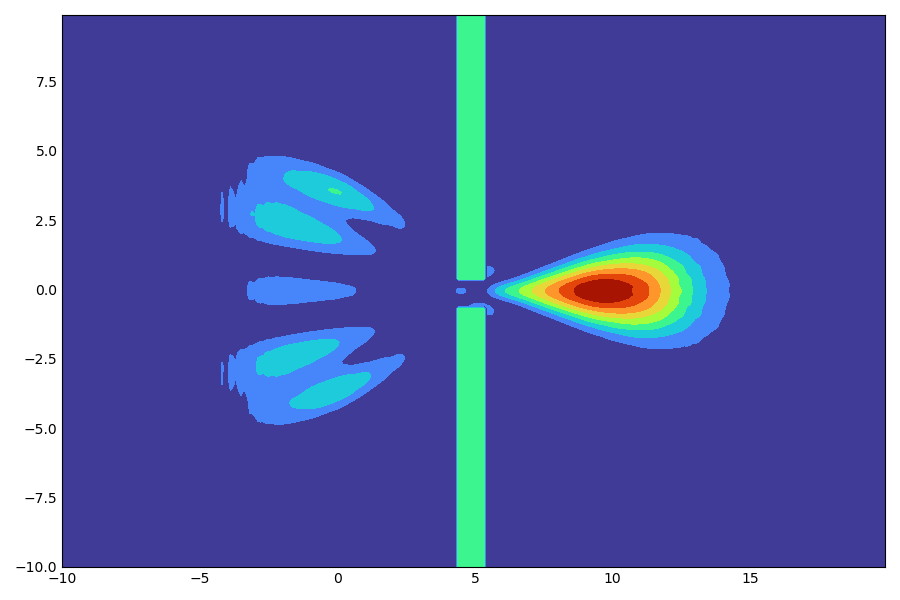
\includegraphics[width=\linewidth]{5/15}
    \end{subfigure}
    \caption{$\Delta y=16\delta,20\delta,30\delta$,t=1100}
\end{figure*}
\onecolumn
\section{Code}
\nolinenumbers
\lstinputlisting[caption=Propagation, language=c]{main.cpp}
\linenumbers
\nolinenumbers
\lstinputlisting[caption=Plot, language=c]{plot.py}
\linenumbers


\twocolumn
\section{Appendix:Tight-Binding propagation method and Application}
\paragraph{} 紧束缚(Tight-Binding,TB)方法是一种在凝聚态物理和量子化学中常用的半经验方法,此方法利用原子轨道构建系统的哈密顿量,利用对角化或非对角化方法研究电子结构。\cite{Li}不同于第一性原理计算方法,紧束缚方法中的哈密顿矩阵由经验参数给出,避免了耗时间较长的自洽场计算\cite{sb}。因此紧束缚方法可以处理较大的体系。利用非对角化的TBPM(Tight-Binding propagation method)方法,可以处理含有数十亿个原子轨道的庞大系统。
\subsection{Methodology}
\subsubsection{Tight-binding models}
\qquad 一个包含n个原子轨道的非周期性系统的哈密顿量可以写成如下形式:
\begin{align}
    \hat{H}=\sum_{i}\epsilon_i c^{\dag}_{i}c_{i}-\sum_{i\neq j}t_{ij}c^{\dag}_{i}c_{j}
\end{align}
可以写成如下紧凑的形式:
\begin{equation}
    \begin{aligned}
        &\hat{H}=\mathbf{c^{\dag}Hc}\\
        &\mathbb{c^{\dag}}=[c^{\dag}_{1},c^{\dag}_{2},\cdots,c^{\dag}_{n}]\\
        &H_{ij}=\epsilon_i\delta_{ij}-t_{ij}(1-\delta_{ij})
    \end{aligned}
\end{equation}
其中$\epsilon_i$称为格位积分(on-site integral),$t_{ij}$为跃迁积分。$c^{\dag},c$为产生湮灭算符。格位积分和跃迁积分的定义为:
\begin{equation}
    \begin{aligned}
        \epsilon_i&=\int \psi^{*}_{i}(r)\hat{h_0}\psi_{i}(r)\dd{r}\\
        t_{ij}&=-\int \psi^{*}_{i}(r)\hat{h_0}\psi_{j}(r)\dd{r}
    \end{aligned}
\end{equation}
$\hat{h_0}$是单粒子的哈密顿量:
\begin{equation}
    \hat{h_0}=-\frac{\hbar^2}{2m}\nabla^2+V(r)
\end{equation}
$\psi_i$是单个原子的原子轨道。在实际的计算中,往往采用Wannier函数。
对具有周期性的体系,利用布洛赫定理,我们可以只关注第一个单胞。为此引入一个额外的指标R:
\begin{equation}
    \psi_{iR}(r)=\psi_i(r-R)
\end{equation}
通过傅里叶变换,定义布洛赫波函数和产生湮灭算符:
\begin{equation}
    \begin{aligned}
        \chi_{ik}(r)=\frac{1}{N}\sum_{R}e^{ik\cdot(R+\tau_i)}\psi_{iR}(r)\\
        c^{\dag}_i(k)=\frac{1}{N}\sum_{R}e^{ik\cdot(R+\tau_i)}c^{\dag}_i(R)\\
        c_i(k)=\frac{1}{N}\sum_{R}e^{-ik\cdot(R+\tau_i)}c_i(R)
    \end{aligned}
\end{equation}
其中N表示单胞的数目。Hamiltonian可以写作:
\begin{equation}
    \hat{H}=N\sum_{k}\{ \sum_{i\in uc}\epsilon_ic^{\dag}_{i}(k)c_i(k)-\sum_{R\neq 0,i\neq j}t_{ij}(R)e^{ik\cdot(R+\tau_i-\tau_j)}c^{\dag}_{i}(k)c_j(k)\}
\end{equation}
\subsubsection{Tight-binding propagation method}
对哈密顿矩阵进行对角化,可以精确地得到特征值和特征态,最终得到所有物理量。然而,精确对角化的内存和CPU时间成本随着模型规模N的增长分别为$O(N^2)$和$O(N^3)$,对于大型的模型来说,这种方法是不可行的。相反,TBPM方法使用一种完全不同的方法处理特征值问题,使得内存和时间消耗与N呈线性关系。\\
在TBPM方法中,初始波函数由一组随机生成的状态组成,然后按如下方程演化:
\begin{equation}
    |\varphi(t)\rangle =e^{-i\hat{H}t}|\varphi(0)\rangle
\end{equation}
关联函数中包含哈密顿量的特征,只要演化时间足够长,演化步长足够小,就可以准确捕捉到哈密顿量的全部特性。最后对关联函数求平均值并进行分析,得到物理量。以DOS的关联函数为例,
\begin{equation}
    C_{DOS}(t)=\langle\varphi(0)|\varphi(t)\rangle
\end{equation}
可以证明它和特征值有以下关系:
\begin{equation}
    \langle\varphi(0)|\varphi(t)\rangle=\sum_{ijk}U_{kj}U_{ij}^{*}a_ia^{*}_{k}e^{-\epsilon_jk}
\end{equation}
$\epsilon_j$是第j个特征值。$U_kj$是第j个特征值的第k个分量。初始波函数写作:
\begin{equation}
    |\varphi(0)\rangle=\sum_{i}a_i|\psi_i\rangle
\end{equation}
其中a是符合归一化$\sum_i |a_i|^2=1$的随机复数。$\psi_i$是基矢量。关联函数可以看作是频率为$\epsilon_i$的波的线性组合。利用逆傅里叶变换,可以确定特征值和DOS。\\
为了演化波函数,需要对时间演化算子进行数值展开,由于TB的哈密顿量是稀疏的,所以可以方便地使用Chebyshev多项式进行展开,这种方法对求解含时薛定谔方程是无条件稳定的。假设$x\in[-1,1]$,
\begin{equation}
    e^{-izx}=J_0(z)+2\sum_{m=1}^{\infty}(-i)^mJ_m(z)T_m(x)
\end{equation}
其中$J_m$是m阶贝塞尔函数,$T_m$是第一类切比雪夫多项式。$T_m(x)$可以由递归关系求解:
\begin{equation}
    T_{m+1}(x)=2xT_{m}-T_{m-1}
\end{equation}
为了利用切比雪夫多项式方法,我们需要将$\hat{H}$缩放为$\tilde{H}=\hat{H}\Vert H\Vert$,使$\tilde{H}$的特征值分布在$[-1,1]$。
\begin{equation}
    |\varphi(t)\rangle=\{J_0(\tau)+2\sum_{m=1}^{\infty}(-i)^mJ_m(\tau)\hat{T}_m(\tilde{H})\}|\varphi(0)\rangle
\end{equation}
$\tau=t\cdot\Vert H\Vert$。在实际计算中不需要存储$\hat{T}_m$,而是由递归关系直接计算波函数:
\begin{equation}
    \hat{T}_{m+1}(\tilde{H})\varphi(0)=2\tilde{H}\hat{T}_{m}(\tilde{H})\varphi(0)-\hat{T}_{m-1}(\tilde{H})\varphi(0)
\end{equation}
除了时间演化算子$e^{-it\hat{H}}$外,其他算子也可以使用类似方法,展开为切比雪夫多项式的级数。
\begin{equation}
    f(x)=\frac{1}{2}c_0T_0(x)+\sum_{m}c_mT_m(x)
\end{equation}
系数定义为
\begin{equation}
    c_m=\frac{2}{\pi}\int_{-1}^{1}\frac{\dd{x}}{\sqrt{1-x^2}}f(x)T_m(x)
\end{equation}
令$x=\cos{\theta}$,并带入上式,可以得到:
\begin{equation}
    \begin{aligned}
        c_m=\frac{2}{\pi}\int_{0}^{\pi}f(\cos{\theta})\cos(m\theta)\dd{\theta}\\
        =Re[\frac{2}{\pi}\sum_{n=0}^{N-1}f(\cos\frac{2\pi n}{N})e^{i\frac{2\pi n}{N}m}]
    \end{aligned}
\end{equation}
因此可以使用快速傅里叶变换计算出$c_k$。以Fermi-Dirac算符为例:
\begin{equation}
    \begin{aligned}
        f(\hat{H})&=\frac{ze^{-\beta\hat{H}}}{1+ze^{-\beta\hat{H}}},\\
        \text{where}\quad\beta&=\frac{1}{k_BT},z=e^{\beta\mu}
    \end{aligned}
\end{equation}
我们定义$\tilde{\beta}=\beta\cdot\Vert\hat{H}\Vert$。根据前面的讨论:
\begin{equation}
    f(\tilde{H})=\sum_{m=0}^{\infty}c_mT_m(\tilde{H})
\end{equation}
\subsection{Application}
\subsubsection{Density of states}
通常计算态密度的方法基于精确对角化,在密集的k网格上获得哈密顿矩阵的特征值,并对特征值求和:
\begin{equation}
    D(E)=\sum_{ik}\delta(E-\epsilon_{ik})
\end{equation}
$\epsilon_{ik}$表示k点的第i个特征值。在实际计算中,$\delta$函数往往用高斯分布函数或洛伦兹分布函数近似:
\begin{align}
    G(E-\epsilon_{ik})&=\frac{1}{\sqrt{2\pi}\sigma}\exp{[-\frac{(E-\epsilon_{ik})^2}{2\sigma^2}]}\\
    L(E-\epsilon_{ik})&=\frac{1}{\pi\sigma}\frac{\sigma^2}{(E-\epsilon_{ik})^2+\sigma^2}
\end{align}
TBPM方法则通过对平均关联函数的逆傅里叶变换计算DOS
\begin{equation}
    D(E)=\frac{1}{2\pi S}\sum_{p=1}^{S}\int_{-\infty}^{\infty}C_{DOS}e^{iEt}\dd{t}
    \label{DOS}
\end{equation}
S是随意初始态的数目。式\ref{DOS}可以通过快速傅里叶变换计算,如果需要更高的能量分辨率,也可以使用数值积分计算。TBPM方法计算DOS的误差随系统增大按照$1/\sqrt{SN}$减少,因此,如果想要更高的精度,可以增大模型尺寸或者计算更多的随机态平均。对于足够大的系统,例如$10^8$个轨道,只需要一组随机初始态就可以得到足够精确的结果。关于DOS计算的更多细节,可以参考这篇文章\cite{PhysRevB.82.115448}。
\subsubsection{Local density of states}
为了计算特定轨道i上的LDOS,我们只将$|\varphi(0)\rangle=\sum_{i}a_{i}\psi_i$中的$a_i$设为非零,然后用与DOS相同的方法对关联函数进行分析。
\begin{align}
    d_i(E)&=\sum_{jk}\delta(E-\epsilon_{jk})|U_{ijk}|^2\\
    \langle \varphi(0)|\varphi(t)\rangle&=\sum_{i}|U_{ijk}a_i|^2e^{-i\epsilon_{j}t}
\end{align}
另一种方法基于Lanczos算法\cite{Haydock_1972},利用递归方法在实空间中评估LDOS。特定轨道i上的LDOS是:
\begin{equation}
    d_i(E)=\lim_{\epsilon\rightarrow 0^+}\frac{1}{\pi}\text{Im}\langle \psi_i|G(E+i\epsilon)|\psi_i\rangle
\end{equation}
然后利用迭代的方法计算出格林函数G(E)的对角元素:
\begin{equation}
    \begin{aligned}
        &G_0=\langle l_0|G(E)|l_0\rangle\\
        &=1/\{E-a_0-b_1^2/[E-a_1-b_2^2/(E-a_3-b_3^2\dots)]\}
    \end{aligned}
\end{equation}
式中的$a_n$和$b_n$由以下的迭代关系求出:
\begin{equation}
    \begin{aligned}
        a_i&=\langle l_i|H_i|l_i\rangle\\
        |m_{i+1}\rangle&=(H-a_i)|l_i\rangle-b_i|l_{i-1}\rangle\\
        b_{i+1}&=\sqrt{\langle m_{i+1}|m_{i+1}\rangle}\\
        |l_{i+1}\rangle&=\frac{|m_{i+1}\rangle}{b_{i+1}}\\
        |l_{-1}\rangle&=|0\rangle
    \end{aligned}
\end{equation}
\subsubsection{Optical conductivity}
\qquad 为了计算光导率,TBPM方法将Kubo公式和随机状态方法相结合。Kubo公式通过时间关联函数(time correlation function)计算系统的宏观响应量。它将微观量(如电导率、磁化率)与系统的时间演化联系起来。对于非相互作用的电子系统,由于在$\beta$方向上的场,在$\alpha$方向上的光学电导率的实部为(省略在$\omega=0$处的Drude贡献)
\begin{equation}
    \begin{aligned}
        \text{Re}&=\lim_{E\rightarrow 0^+}\frac{e^{-\beta \hbar \omega}-1}{\hbar\omega A}\int_{0}^{\infty}e^{-Et}sin(\omega t)\\ &\times 2\text{Im}\langle\psi|f(H)J_{\alpha}(t)[1-f(H)]J_{\beta}|\psi\rangle \dd{t}
        \label{sigma}
    \end{aligned}
\end{equation}
A是系统的面积或者体积。对于紧束缚的哈密顿量,流密度算符定义为:
\begin{equation}
    J=-\frac{ie}{\hbar}\sum_{i,j}t_{ij}{\hat{r_j}-\hat{r_i}c^{\dag}_ic_j}
\end{equation}
$\hat{r}$是位置算符。Fermi-Dirac贡献,定义为:
\begin{align}
    f(H)=\frac{1}{e^\beta{H-\mu}-1}
\end{align}
在实际的计算中,通过对实空间的所有基态的随机叠加,确保\ref{sigma}的精度。Fermi-Dirac算符,如前面所述,可以利用切比雪夫多项式和快速傅里叶变换计算。我们引入两个波函数:
\begin{equation}
    \begin{aligned}
        |\psi_1(t)\rangle=e^{-i\tilde{H}t}[1-f(\tilde{H})]J_{\alpha}|\psi(0)\rangle\\
        |\psi_2(t)\rangle=e^{-i\tilde{H}t}f(\tilde{H})|\psi(0)\rangle\\
    \end{aligned}
\end{equation}
于是可得$\sigma_{\alpha\beta}(t)$的实部:
\begin{equation}
    \begin{aligned}
        \text{Re}&=\lim_{E\rightarrow 0^+}\frac{e^{-\beta \hbar \omega}-1}{\hbar\omega A}\int_{0}^{\infty}e^{-Et}sin(\omega t)\\ &\times 2\text{Im}\langle\psi_2|J_{\alpha}(t)|\psi\rangle_{\beta} \dd{t}
        \label{sigma}
    \end{aligned}
\end{equation}
由KK(Kramers-Kronig)关系,推导出$\sigma_{\alpha\beta}$的虚部:
\begin{equation}
    \text{Im}\sigma_{\alpha\beta}(\hbar\omega)=-\frac{1}{\pi}P\int_{-\infty}^{\infty}\frac{\text{Re} \sigma_{\alpha\beta}(\hbar\omega')}{\omega'-\omega}\dd{\omega}
\end{equation}
\subsubsection{DC conductivity}
直流电导率可以通过$\lim \omega\rightarrow0$时的Kubo公式来计算。基于之前的DOS和准本征态计算方法,T=0时,直流电导率在$\alpha$方向上的对角线项为:
\begin{equation}
    \begin{aligned}
        \sigma_{\alpha\alpha}(E)&=\lim_{\tau\rightarrow\infty}\sigma_{\alpha\alpha}(E,\tau)\\
        &=\lim_{\tau\rightarrow\infty}\frac{D(E)}{A}\int_{0}^{\tau}\text{Re}[e^{-iEt}C_{DC}(t)]\dd{t}
    \end{aligned}
\end{equation}
其中DC关联函数定义为:
\begin{equation}
    C_{DC}=\frac{\langle\psi(0)|J_{\alpha}e^{-i\tilde{H}t}J_{\alpha}|\tilde{\Psi}(E)\rangle}{\langle\psi(0)|\tilde{\Psi}(E)\rangle}
\end{equation}
A表示面积或者体积。需要强调的是,$|\psi(0)\rangle$必须与计算$|\tilde{\Psi}(E)\rangle$时所用的随机初始态相同。不考虑安德森局域化影响的半经典直流电导率定义为:
\begin{equation}
    \sigma^{sc}=\sigma^{max}_{\alpha\alpha}(E,\tau)
\end{equation}
实验中测量的场效应载流子迁移率与半经典直流电导率有关:
\begin{equation}
    u(E)=\frac{\sigma^{sc}}{en_{e}(E)}
\end{equation}
其中载流子密度可以由态密度的积分求出:
\begin{equation}
    n_{e}=\int_{0}^{E}D(\varepsilon)\dd{\varepsilon}
\end{equation}
\subsubsection{Diffusion coefficient}
根据Kubo公式,直流电导率也可以写成扩散系数的函数:
\begin{equation}
    \sigma_{\alpha\alpha}(E)=\frac{e^2}{A}D(E)\lim_{\tau\rightarrow\infty}D_{diff}(E,\tau)
\end{equation}
因此,可以反推出扩散系数的计算方法:
\begin{equation}
    D_{diff}=\frac{1}{e^2}\int_{0}^{\tau}e^{-iEt}C_{DC}(t)\dd{t}
\end{equation}
一旦求出了扩散系数,就可以立即得到载流子速率:
\begin{equation}
    v(E)=\sqrt{D_{diff(E,\tau)}/\tau}
\end{equation}
以及平均自由程、安德森局域长度等物理量。

\newpage
%\clearpage%新一页而不是新一列

	
%    If line numbering is enabled, we recommend placing the command \verb|\nolinenumbers| at the beginning %and \verb|\linenumbers| at the end of the code. 
%	
%    This will temporarily remove line numbering and the code will look better as shown in this example.

%----------------------------------------------------------
\nocite{*}
\addcontentsline{toc}{section}{References}

\printbibliography

%----------------------------------------------------------
%\section{Document style options}
%
%    \subsection{Tau start}
%	
%        We included the \verb|\taustart{}| command, which provides a personalized lettrine for the %beginning of a paragraph.
%
%    \subsection{Line numbering}
%	
%        By implementing the \textit{lineno} package, the line numbering of the document can be placed with %the command \verb|\linenumbers|.
%		
%        I recommend placing the command after the abstract and table of contents for a better appearance.
%		
%    \subsection{Table of contents}
%	
%        The \textit{tau class} provides a customised design for the table of contents. Each level of the %ToC provides a preview of the content and its location in the document. 
%		
%section{Figures and tables}
%
%   \subsection{Figures}
%		
%	Fig. \ref{fig:figure} shows an example figure.
%		
%	\begin{figure}[H]
%		\centering
%		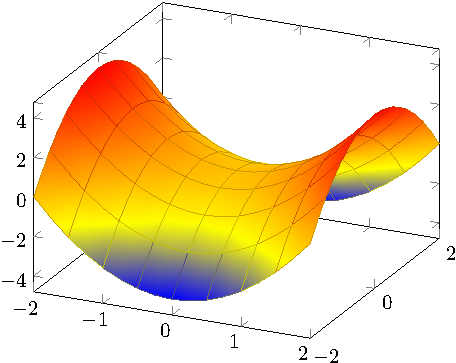
\includegraphics[width=0.75\columnwidth]{figures/Example.pdf}
%		\caption{Example figure obtained from PGFPlots \cite{PFGPlots}.}
%		\label{fig:figure}
%	\end{figure}
%		
%       Fig. \ref{fig:examplefloat} shows an example of two figures that covers the width of the page. It can be placed at the top or bottom of the page. The space between the figures can also be changed using the \verb|\hspace{Xpt}| command.
%		
   
	
%    \subsection{Tables}
%	
%        Table \ref{tab:table} shows an example table. The \verb|\tabletext{}| is used to add notes to %tables easily. 
%		
%	\begin{table}[H]
%		\centering
%		\caption{Small example table.}
%		\label{tab:table}
%		\begin{tabular}{cc}
%			\toprule
%			\textbf{Column 1} & \textbf{Column 2} \\
%			\midrule
%			Data 1 & Data 2 \\
%			Data 3 & Data 4 \\
%			\bottomrule
%		\end{tabular}
%			
%            \tabletext{Note: I'm a table text for additional information.}
%			
%	\end{table}
%		
%\section{Tau packages}
%
%    \subsection{Tauenvs}
%	
%		
%	\begin{tauenv}[frametitle=Environment with custom title]
%            This is an example of the custom title environment. To add a title type \verb|[frametitle=Your %title]| next to the beginning of the environment (as shown in this example).
%	\end{tauenv}
%
%		
%\section{Equation}
%
%    Equation \ref{ec:equation}, shows the Schrödinger equation as an example. 
%	\begin{equation} \label{ec:equation}
%		\frac{\hbar^2}{2m}\nabla^2\Psi + V(\mathbf{r})\Psi = -i\hbar \frac{\partial\Psi}{\partial t}
%	\end{equation} 
\end{document}